\documentclass{article}
\usepackage[T1]{fontenc}
\usepackage{lmodern}
\usepackage{graphicx}
\usepackage{amsmath,amssymb}
\usepackage[a4paper,margin=2cm]{geometry}
\usepackage[absolute,overlay]{textpos}
\setlength{\TPHorizModule}{1mm}
\setlength{\TPVertModule}{1mm}
\usepackage[indonesian]{babel}
\usepackage{hyperref}
\setlength{\emergencystretch}{2em}
% unit: Halaman 44

\begin{document}

% === Halaman 44 (llm) ===

% (tidak ada teks dari model)

% deskripsi: Screenshot kode program Python yang mengimplementasikan enkripsi dan dekripsi menggunakan Vigenere Cipher, lengkap dengan input pengguna dan output hasil eksekusi.
% bbox normalisasi: [0.0600, 0.1700, 0.9300, 0.8400]
\begin{textblock*}{182.70mm}(12.60mm,50.49mm)
\noindent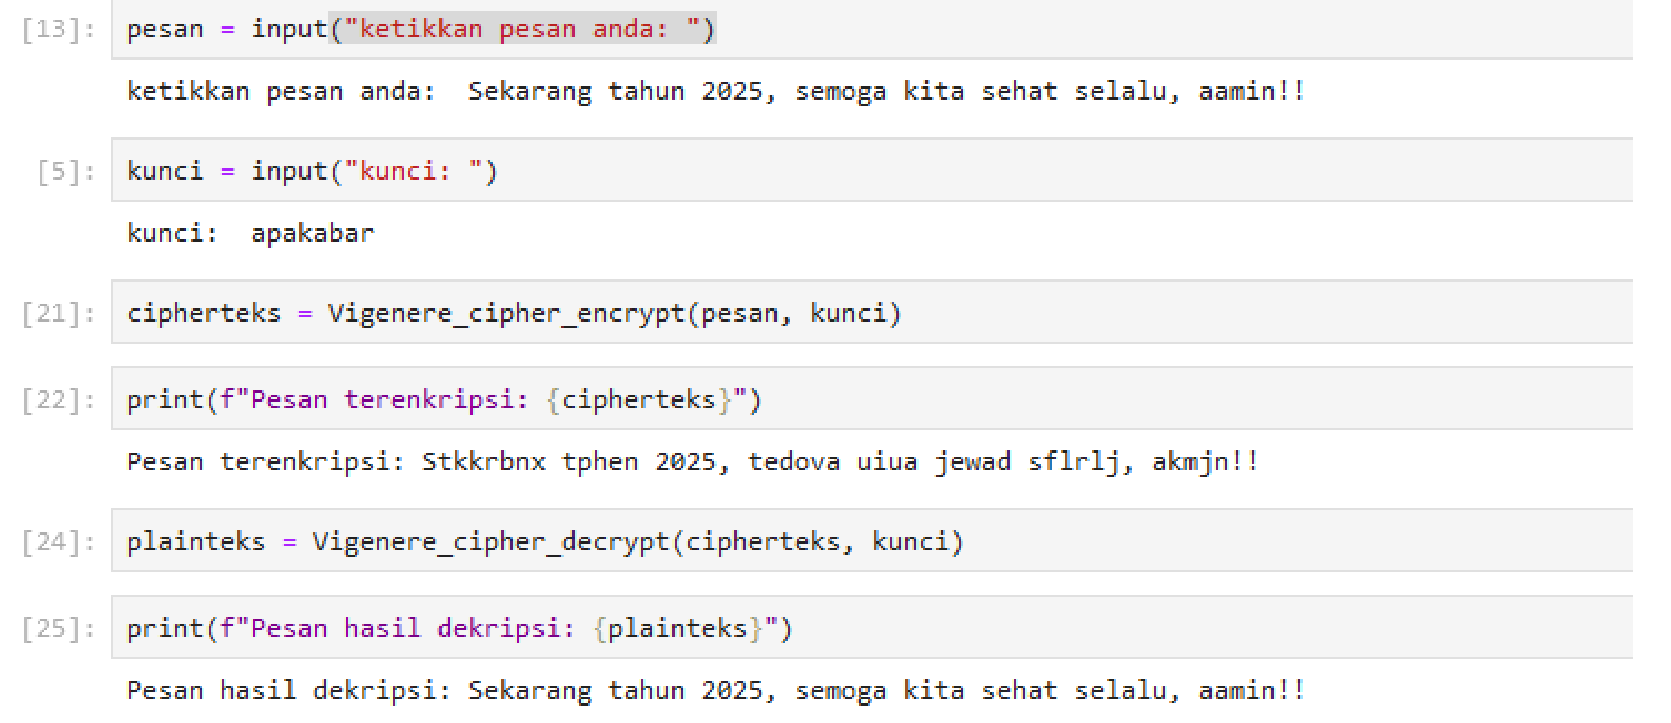
\includegraphics[width=182.70mm,height=198.99mm]{../../images/llm/page_044_img_01.png}%
\end{textblock*}

\end{document}
